\chapter{Case Study: The University of Brasília Herbarium (UB) dataset}\label{casestudy_ub}
% herbarium page: http://florescer.unb.br/bol/
% Add herbarium historical

In this section I describe the application of the network models for deriving enriched information from the University of Brasilia Herbarium (UB) dataset.
The UB Herbarium is physically based at the University of Brasília Biology Department (UnB-IB) since its foundation in 1963.
The dataset is made publicly available for download through the Global Biodiversity Information Facility (GBIF) portal.
Here I assume the dataset has already been passed through a data cleaning process, and the entity resolution problem resolved.
Both CWN and SCN were built for supporting data enrichment.
Routines were written in Python3, using the Networkx and Pandas libraries.


Collectors had historical contributions to the herbarium \ref{table:ub_collectors_florescer}.

\begin{table}[H]
  \caption{Historically important collectors in the UB herbarium.}
  \begin{center}
  \begin{tabular}{l c c}
      & activity years & contribution\\
      \hline
      William R. Anderson & 1962-1976 & Central Brazil Expedition (NY Botanical Garden)\\
      Howard S. Irwin & 1962-1976 & Central Brazil Expedition (NY Botanical Garden)\\
      George Eiten & - & Cerrado biome, mainly in MA state \\
      James Alexander Ratter & 
      	\begin{tabular}[t]{{@{}c@{}}}1968-1976 \\ 1996-2006\end{tabular} &
        \begin{tabular}[t]{{@{}c@{}}}Xavantina-Cachimbo expedition \\ Cerrado biome\end{tabular} \\
      Joseph Harold Kirkbride Junior & 1976-1983 & Flora of DF \\
      Ana Lúcia Tostes Leite & 1982-1984 & Continental algae of DF \\
      Carolyn Elinores Barnes Proença & 1981-current & Cerrado biome \\
      Maria das Graças Machado de Souza & 1982-current & Continental algae of DF and GO\\
      \hline
  \end{tabular}
  \\[1.5em]
  \hfill Source: FLORESCER Project webpage \cite{florescer}
  \end{center}
  \label{table:ub_collectors_florescer}
\end{table}

\section{Dataset Characterization}

%%%%%%%%%%%%%%%%%%%%%%%%%%%%%
%% Taxonomic characterization

After loading the dataset with specified columns into memory I've filtered out records with missing values for fields \textit{recordedBy} or \textit{scientificName}, as these are critical for building the network models.
At the time of this study the resulting dataset had a total of 185301 records. However not all records have been identified up to the taxonomic resolution of \textit{species}, as shown in Table \ref{table:dset_taxonomicres_counts}. 
As taxons hold a tree-like hierarchical relationship, those at more inclusive (broader) ranks can be successfully derived from more restrictive ones, but not the inverse. Each child taxon have exactly one parent, but a parent taxon can have one or more children.
To give an example, the table shows that approximately $76\%$ of the records are at the resolution of species. However the species identity of records at higher resolutions, in this case form or variety, are automatically determined by following parental paths. This makes species identity derivable for approximately $82\%$ of the records, as shown in the cumulative percentage for the species rank.

For the construction of SCNs we must make sure only to include records that were identified up to the same taxonomic resolution as the model itself, keeping in mind that lower-resolution entities can be derived from higher-resolution ones. 
For CWNs, on the other hand, the taxonomic resolution of each record is not relevant for model construction, as edges are built using only collector cliques. In this case all records with at least two collectors can be used, irrespective of their taxonomic resolution.

\begin{table}[H]
  \caption{Number of records with maximum taxonomic resolution at each rank. Ranks are ordered hierarchically, being \textit{FORM} the most restrictive (higher resolution) and \textit{KINGDOM} the broader (lower resolution) one. Cumulative metrics show the total amount of records that could be derived for each rank.}
  \begin{center}
  \begin{tabular}{l c c c c}
       & count & \% & cumulative count & cumulative \% \\
      \hline
      FORM & 1000 & 0.5397 & 1000 & 0.5397\\
      VARIETY & 8935 & 4.8219 & 9935 & 5.3615\\
      SUBSPECIES & 1681 & 0.9072 & 11616 & 6.2687\\
      SPECIES & 140763 & 75.9645 & 152379 & 82.2332\\
      GENUS & 24397 & 13.1661 & 176776 & 95.3994\\
      FAMILY & 6223 & 3.3583 & 182999 & 98.7577\\
      PHYLUM & 294 & 0.1587 & 183293 & 98.9164\\
      KINGDOM & 2008 & 1.0836 & 185301 & 100\\
      \hline
      total & 185301 & 100 & &
  \end{tabular}
  \end{center}
  \label{table:dset_taxonomicres_counts}
\end{table}

% what are the main families?

\begin{table}[H]
  \caption{Number of distinct taxons at each taxonomic rank in the dataset. For each rank a list with its top-5 most recorded taxons is included with their respective counts.}
  \begin{center}
  \begin{tabular}{l c c c}
   & num of taxons & top-5 taxons & num of records \\
   \hline
    kingdom & 5 &
	\begin{tabular}[t]{{@{}c@{}}}Plantae\\Chromista\\Fungi\\Bacteria\end{tabular} &
	\begin{tabular}[t]{{@{}r@{}}}179218\\4204\\1391\\342\end{tabular} \\ \\
    phylum & 12 &
	\begin{tabular}[t]{{@{}c@{}}}Tracheophyta\\Bryophyta\\Ochrophyta\\Charophyta\end{tabular} &
	\begin{tabular}[t]{{@{}r@{}}}153589\\16485\\4133\\3500\end{tabular} \\ \\
    class & 29 &
	\begin{tabular}[t]{{@{}c@{}}}Magnoliopsida\\Liliopsida\\Bryopsida\\Bacillariophyceae\end{tabular} &
	\begin{tabular}[t]{{@{}r@{}}}126288\\23004\\15899\\4133\end{tabular} \\ \\
    order & 136 &
	\begin{tabular}[t]{{@{}c@{}}}Myrtales\\Fabales\\Poales\\Malpighiales\end{tabular} &
	\begin{tabular}[t]{{@{}r@{}}}24312\\20846\\17159\\16188\end{tabular} \\ \\
    family & 507 &
	\begin{tabular}[t]{{@{}c@{}}}Fabaceae\\Myrtaceae\\Asteraceae\\Rubiaceae\end{tabular} &
	\begin{tabular}[t]{{@{}r@{}}}19254\\12833\\11271\\9447\end{tabular} \\ \\
    genus & 3374 &
	\begin{tabular}[t]{{@{}c@{}}}Myrcia\\Eugenia\\Mimosa\\Miconia\end{tabular} &
	\begin{tabular}[t]{{@{}r@{}}}4654\\3750\\2992\\2402\end{tabular} \\ \\
    species & 15379 &
	\begin{tabular}[t]{{@{}c@{}}}\textit{Myrcia splendens}\\\textit{Myrcia guianensis}\\\textit{Eugenia punicifolia}\\\textit{Sematophyllum subpinnatum}\end{tabular} &
	\begin{tabular}[t]{{@{}r@{}}}696\\560\\462\\438\end{tabular} \\
  \hline
  \end{tabular}
  \end{center}
  \label{table:taxons}
\end{table}

%%%%%%%%%%%%%%%%%%%%%%%%%%%%%%
%% Geographic characterization

From the set of $185301$ records approximately $48\%$ (a total of $89216$) were interpreted and tagged as having geospatial issues during internal preprocessing routines in the \textit{GBIF} platform \cite{GBIF.ORG}.
During geospatial validation the routines check for each record ($i$) if geographical coordinates are erroneously assigned to zero latitude and longitude; ($ii$) if geographic coordinates are in fact placed within the boundaries of the country if indicated; and ($iii$) if lat/long values are likely to having been swapped or negated during recording.
If inconsistencies are detected during the execution of such routines, issues are registered for each record, priorly to making the dataset available for download or query via API. 
% http://www-old.gbif.org/infrastructure/processing

As shown in Figure \ref{fig:venn_geospatial_issues} most geospatial issues are due to records being assigned to zero coordinates (zero latitude and longitude), which also makes them laying outside of the country boundaries. As a consequence they are tagged as having both the ``Zero Coordinates'' (ZC) and ``Country Coordinates Mismatch'' (CCM) issues, being represented in the figure as the intersection between CCM and ZC.
Some records with only the CCM issue were not misplaced in coordinates $(0,0)$, but still were improperly placed outside the country frontiers. 
On the other hand, records with only the ZC issue are those which were misplaced in coordinates $(0,0)$ but were lacking information about the country, and therefore couldn't be classified as being outside the country frontiers.

  \begin{figure}[h!]
  	\centering
    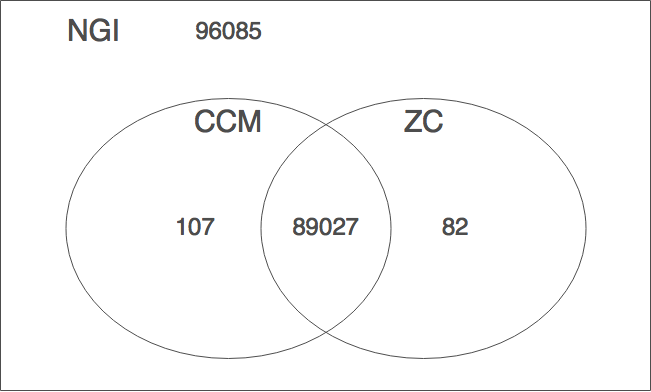
\includegraphics[width=0.6\linewidth]{figures/venn_geospatial_issues.png}
    \caption{Number of occurrences from the UB herbarium dataset classified within each geospatial issue class. \textit{NGI}: Records with no geospatial issues; \textit{CCM}: Country Coordinates Mismatch issue; \textit{ZC}: Zero Coordinates issue.}
    \label{fig:venn_geospatial_issues}
  \end{figure}

Records without geospatial issues comprise approximately $52\%$ of the dataset, and their coordinates are shown in Figure \ref{fig:occurrence_map}. Notice that the figure extent is constrained around the Brazilian territory, and records outside the canvas are omitted. Although most records deposited in the UB herbarium were collected in Brazil, there is also a considerable amount of records from many other countries (Figure \ref{fig:recs_by_cntry_state}a), that were been obtained from herbaria exchange activities or international recording expeditions. According to the herbarium description available from the \textit{Florescer project} webpage \cite{florescer}, records from the Amazon and Atlantic forest were mostly exchanges under the curatorship of \textit{Dr. João Murça Pires} and \textit{Dr. Graziela Maciel Barroso}, respectively. A considerable part of international records were exchanges incorporated under the curatorship of \textit{Dr. George Eiten}.  


  \begin{figure}[!htb]
  	\centering
    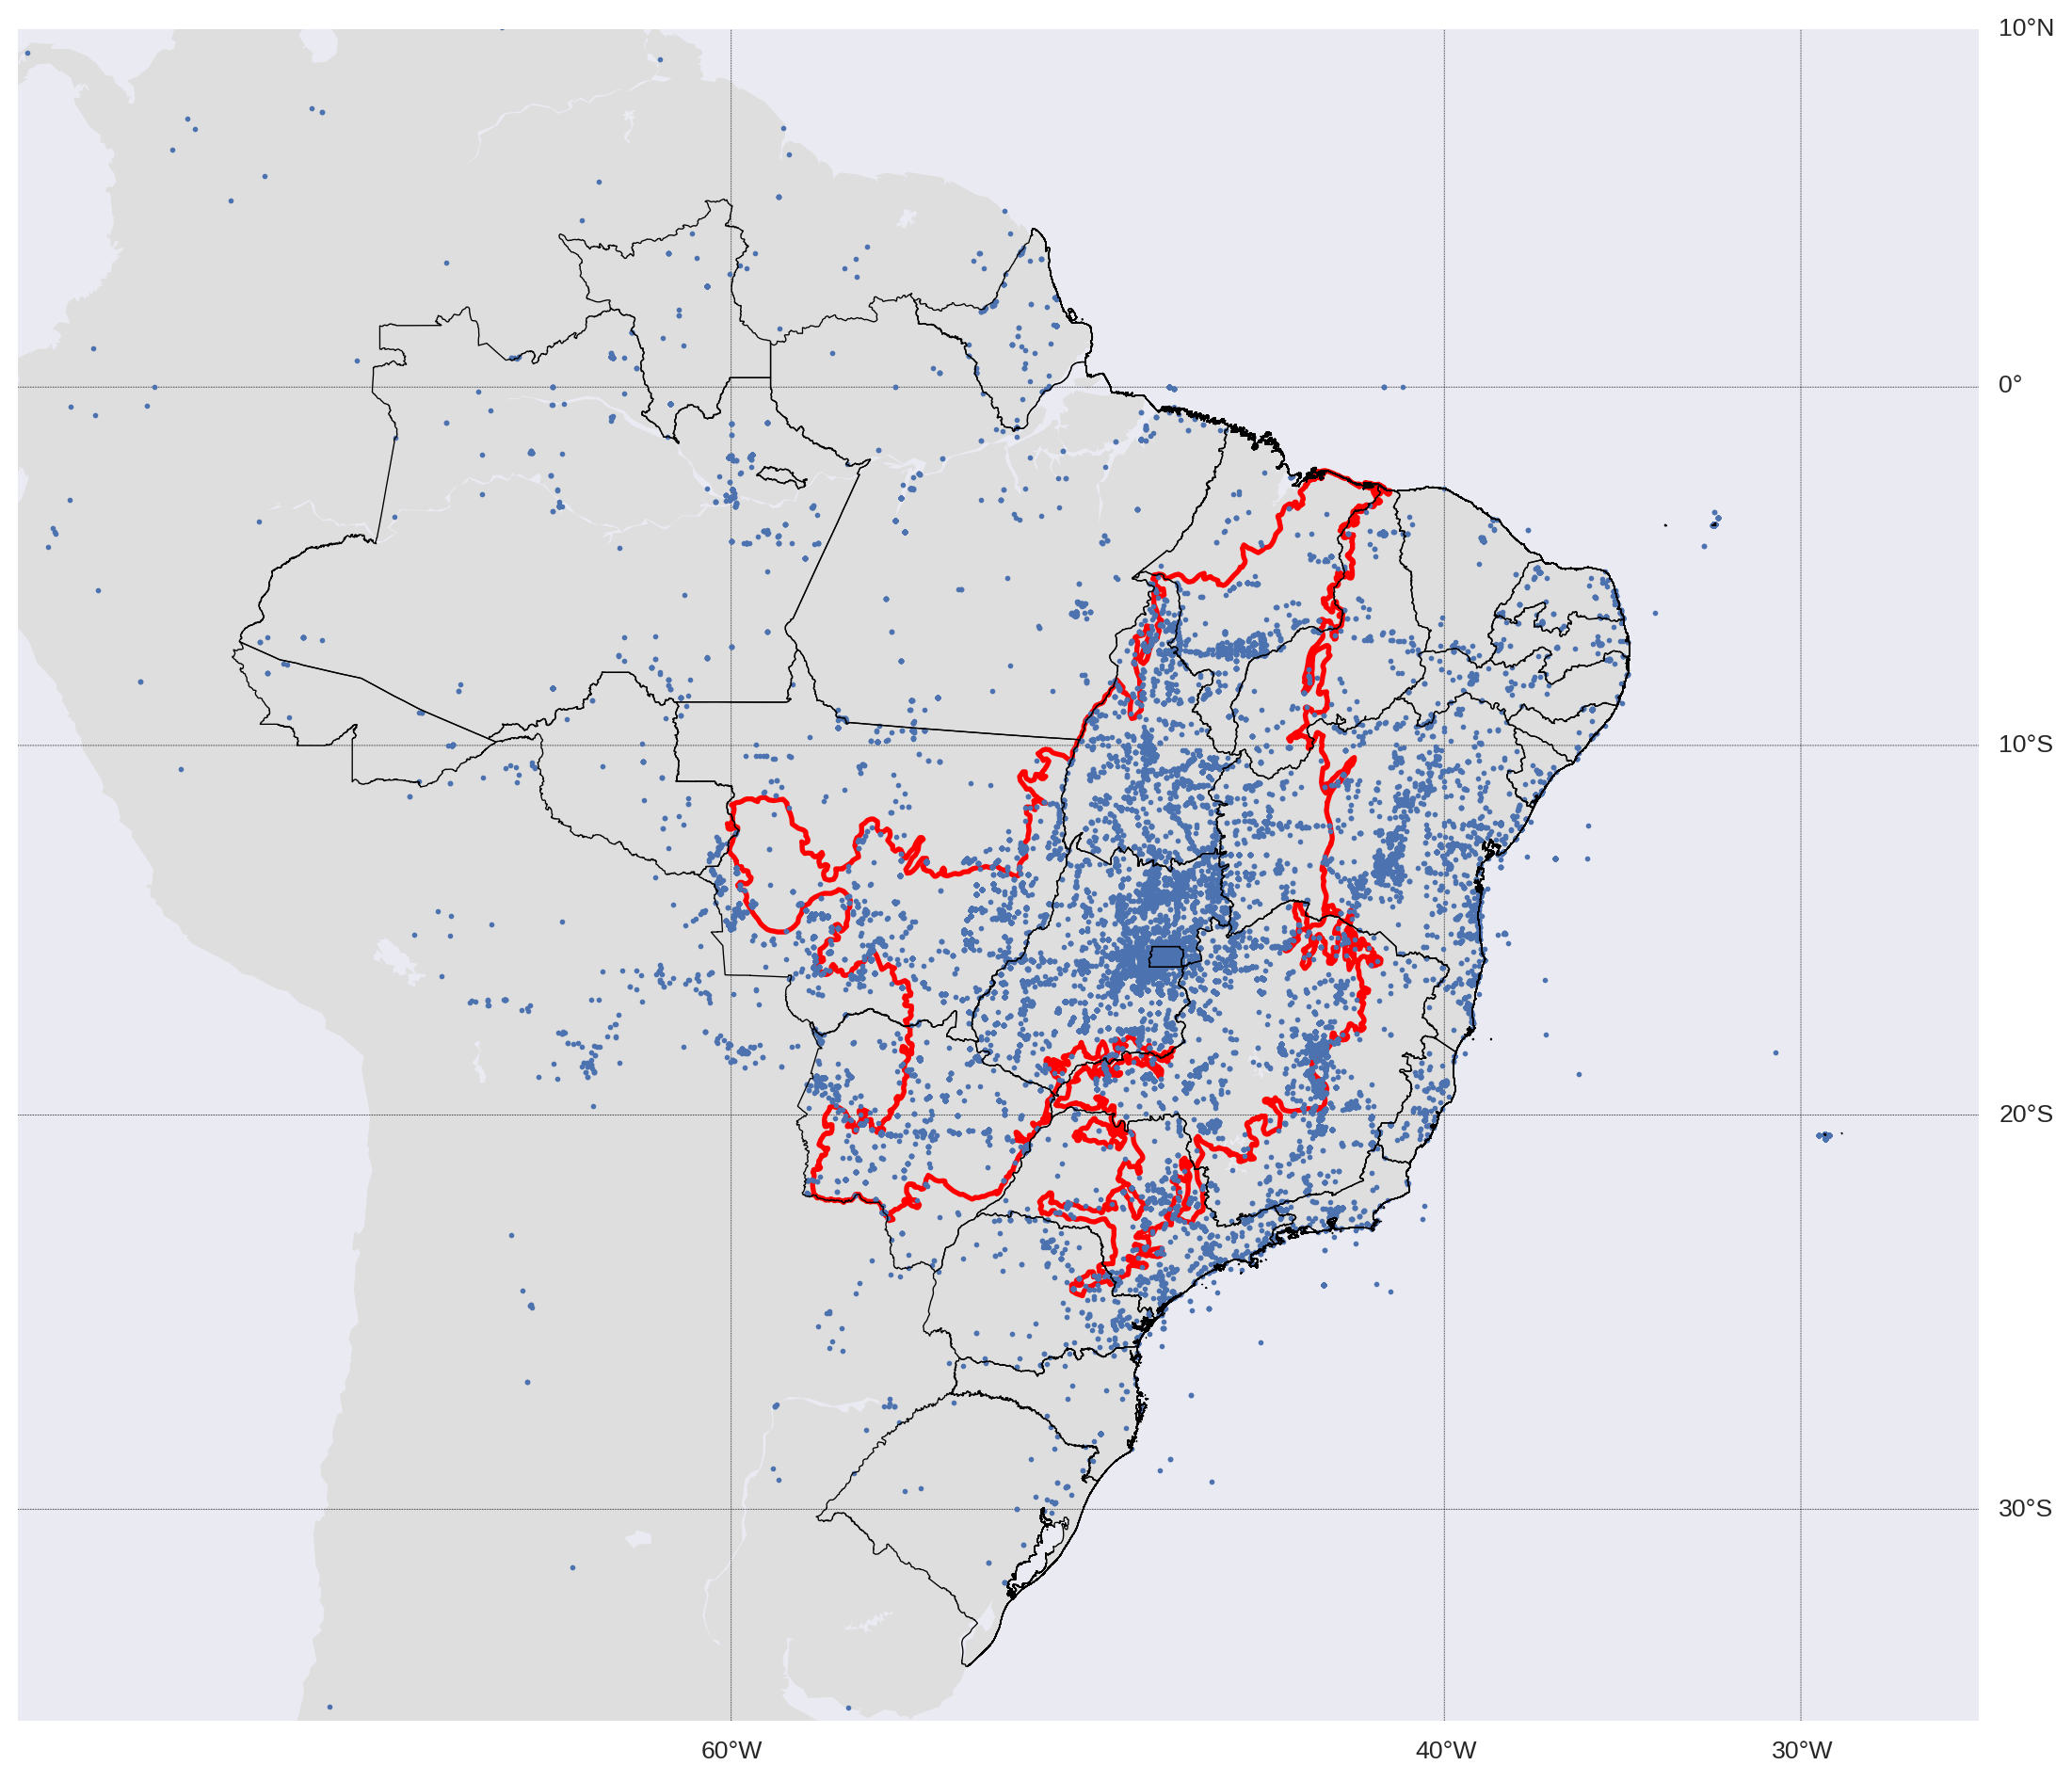
\includegraphics[width=\linewidth]{figures/occurrence_map.png}
    \caption{Geographic distribution of the occurrences from the UB Herbarium dataset near the Brazilian territory. Records without geospatial issues are placed in the map as blue dots. The area outlined in red represents the boundaries of the Cerrado biome.}
    \label{fig:occurrence_map}
  \end{figure}
  
  \begin{figure}[!htb]
  	\centering
    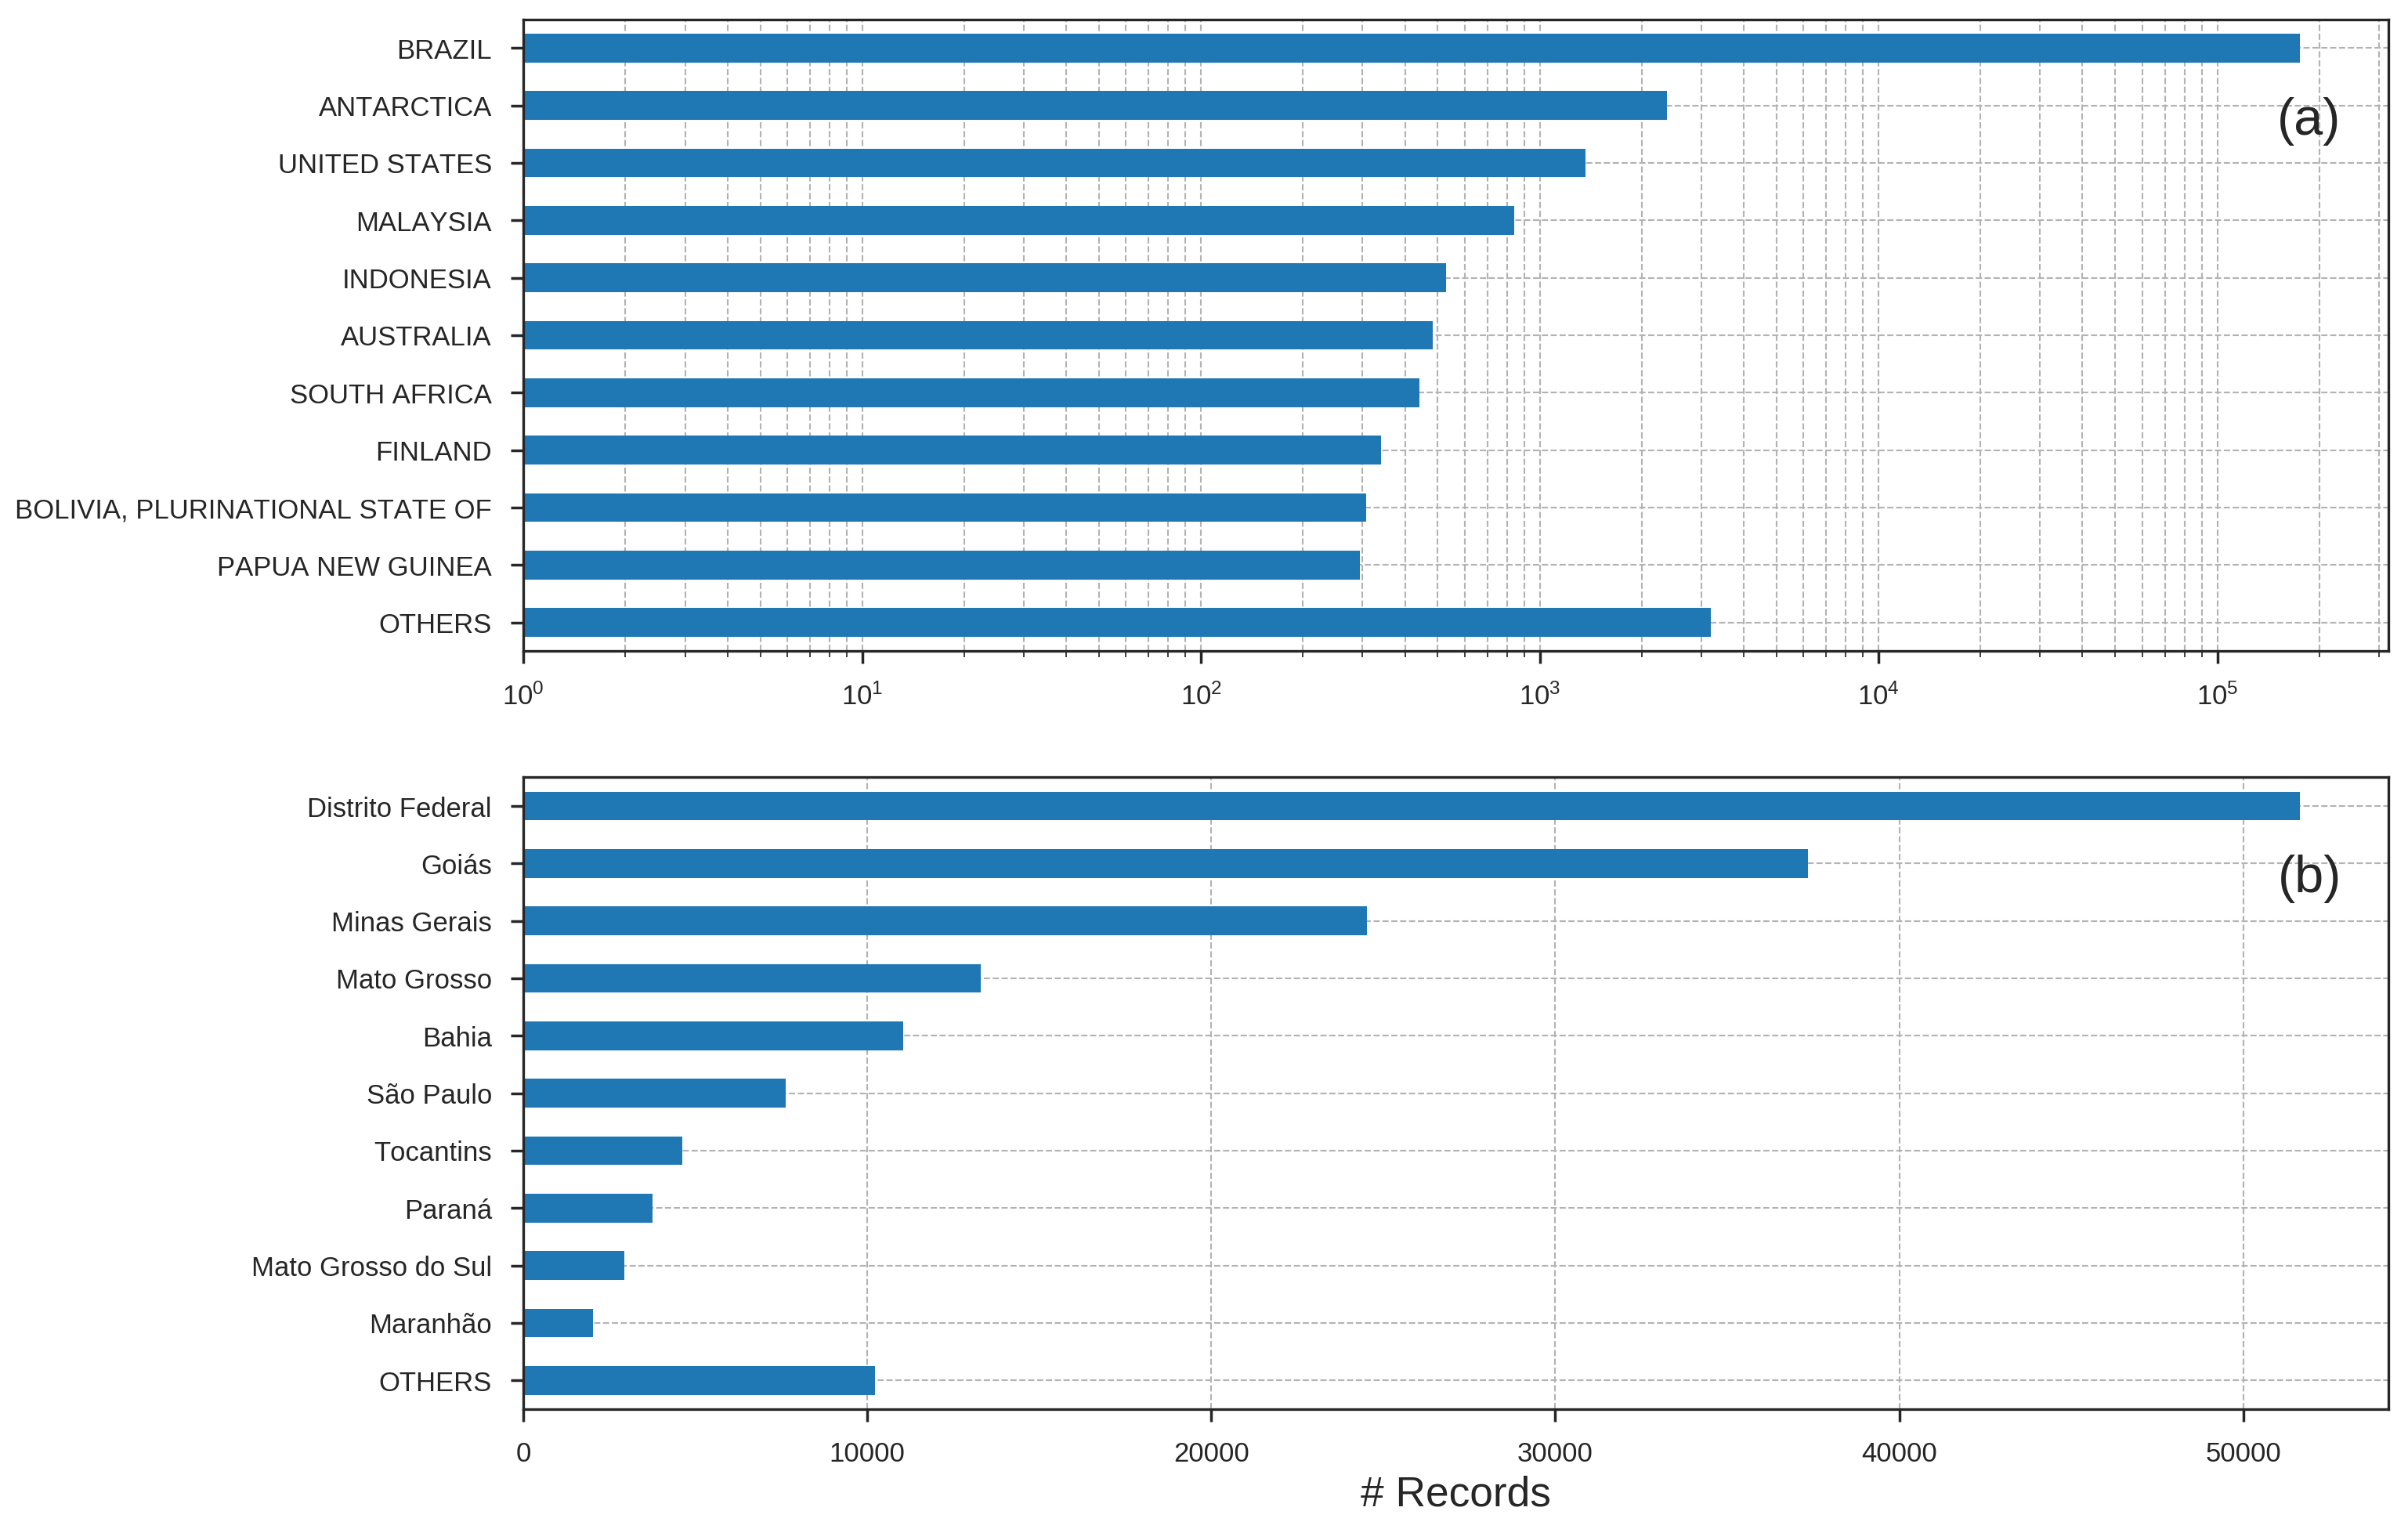
\includegraphics[width=\linewidth]{figures/recs_by_cntry_state.png}
    \caption{Top-10 countries (a) and top-10 Brazilian states (b) with most occurrence records deposited in the UB herbarium. Records from countries and states beyond the $10th$ position in the respective ranks are summed and assigned to \textit{OTHERS}.}
    \label{fig:recs_by_cntry_state}
  \end{figure}
  
Within the Brazilian territory, the Federal District was the most sampled federative unit despite its small area, followed by the state of Goiás (\ref{fig:recs_by_cntry_state}b). 
Such a geographic bias in the occurrences distribution can be explained by the fact that UB is physically located in the University of Brasilia, making it more viable for associated collectors to record in nearby locations.
Moreover, as UB is a national reference herbarium for species occurring the Cerrado biome, botanists working in Cerrado areas become more inclined to deposit their recordings in the institution.
In fact, figure \ref{fig:occurrence_map} shows that UB records are more densely concentrated within the Cerrado biome, mostly in the Central Brazil region. 


  
%%%%%%%%%%%%%%%%%%%%%%%%%%%%
%% Temporal characterization
Almost $98\%$ of the records contain information about their collection dates.
The oldest records in the herbarium dataset date from 1800.
However, more intensive collection activity started around 1960. Around 8000 records in the herbarium date up to that time (Figure \ref{fig:ub_records_timeseries}(c)). 
From 1950 to present, there are two apparent peaks in collection activity around year 1965 and 2013 (Figure \ref{fig:ub_records_timeseries}(a)). % Why?

  \begin{figure}[h!]
  	\centering
    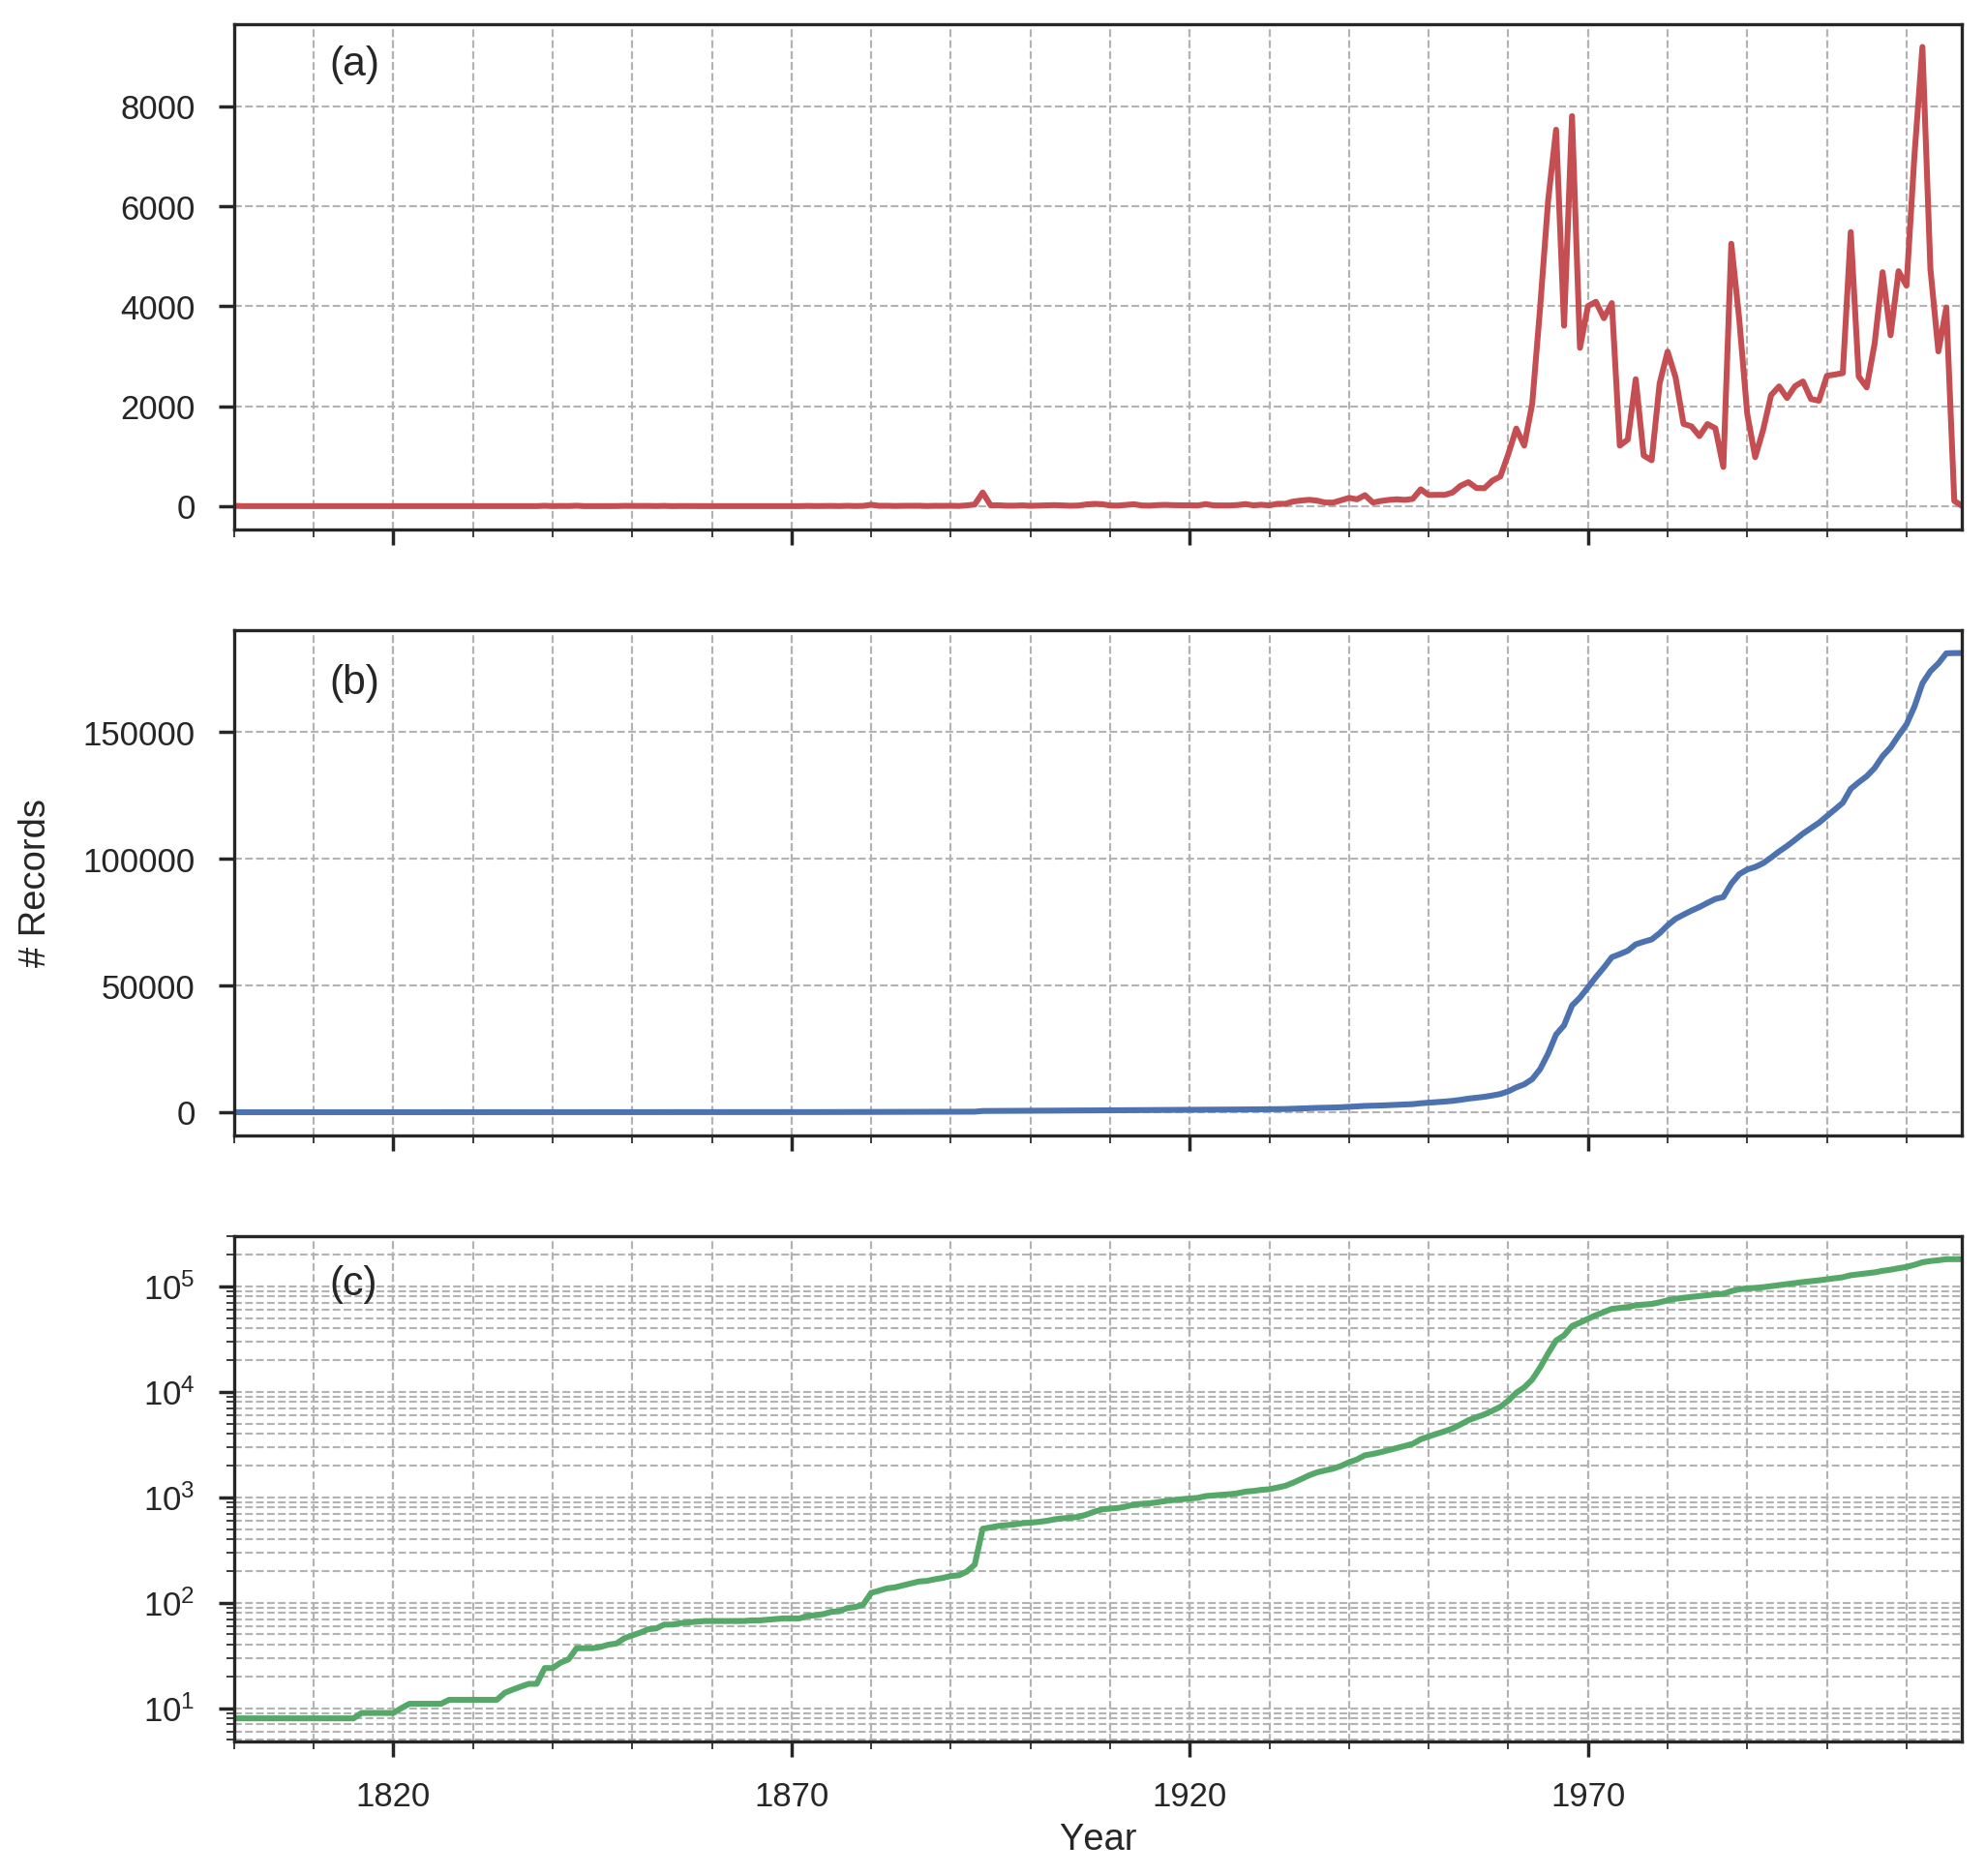
\includegraphics[width=\linewidth]{figures/ub_records_timeseries.png}
    \caption{Recording activities registered in the UB herbarium since 1800, aggregated by year. (a) Absolute record counts for each year. (b) Cumulative counts of records in a linear scale. (c) Cumulative counts of records using a logarithmic scale.}
    \label{fig:ub_records_timeseries}
  \end{figure}


\section{Network models construction}
%%%%%%%%%%%%%%%%%%%%%%%%%%%%%%
%%%%%%%%%%%%%%%%%%%%%%%%%%%%%%
%% Network models construction


% Build SCN
% What is the species with more collectors? What is the collector with more species?
% Average collector/species & species/collector  (with percentages)

\newcommand{\ubNumSpNodes}{15344}
\newcommand{\ubNumColNodes}{6768}
For exploring the recording behavior of UB collectors in terms of their taxonomic preferences we initially built a Species-collectors network model (SCN), linking collectors to the species they've recorded. 
Some data preprocessing routines including names atomization and null values filtering were were executed in the tabular dataset before it could be used to build the model.
Additionally, a previously elaborated names map for the UB dataset collectors was passed in during SCN construction, facilitating the process of remapping names variants to entities. 
Finally, nodes derived from noise entities such as \textit{``et. al"}, \textit{``Incógnito"}, \textit{``Ignorado"}, \textit{``Ilegível"} and \textit{``?"} were excluded from the network model right after its creation.
The resulting network had a total of $\ubNumSpNodes$ species and $\ubNumColNodes$ collectors nodes.

By inspecting the degree distribution of nodes from both species and collectors sets (Figure \ref{fig:ub_scn_degree_dist}) one can notice that the network is majoritarily composed by nodes holding very few ties with others, while few others, called hubs, are very intensely connected. 
In fact a total of $12123$ species, comprising $79\%$ of all species nodes, are linked to $10$ or fewer collectors, while conversely around $79\%$ of all collectors (a total of $5362$ nodes) are linked to $10$ of fewer species. 
As opposed to random networks, in which extremely well or extremely poorly connected nodes are very unlikely to occur, the connectivity pattern observed for the UB species-collectors network resembles the one from scale-free networks. While the degree distribution in random networks follow a poisson distribution, in scale-free networks it is better described by a power law $ p(k) \sim k^{-\alpha} $. For some empirical datasets, as it is the case for the $S_{sp}$ nodes set, a slight variant of the power law function $p(k) \sim e^{-\lambda k} k^{-\alpha}$ can turn out to be a better fit. The additional exponential term is the cutoff term, which is responsible for the tail cutoff that can be observed in Figure \ref{fig:ub_scn_degree_dist}a. 

  \begin{figure}[!h]
  	\centering
    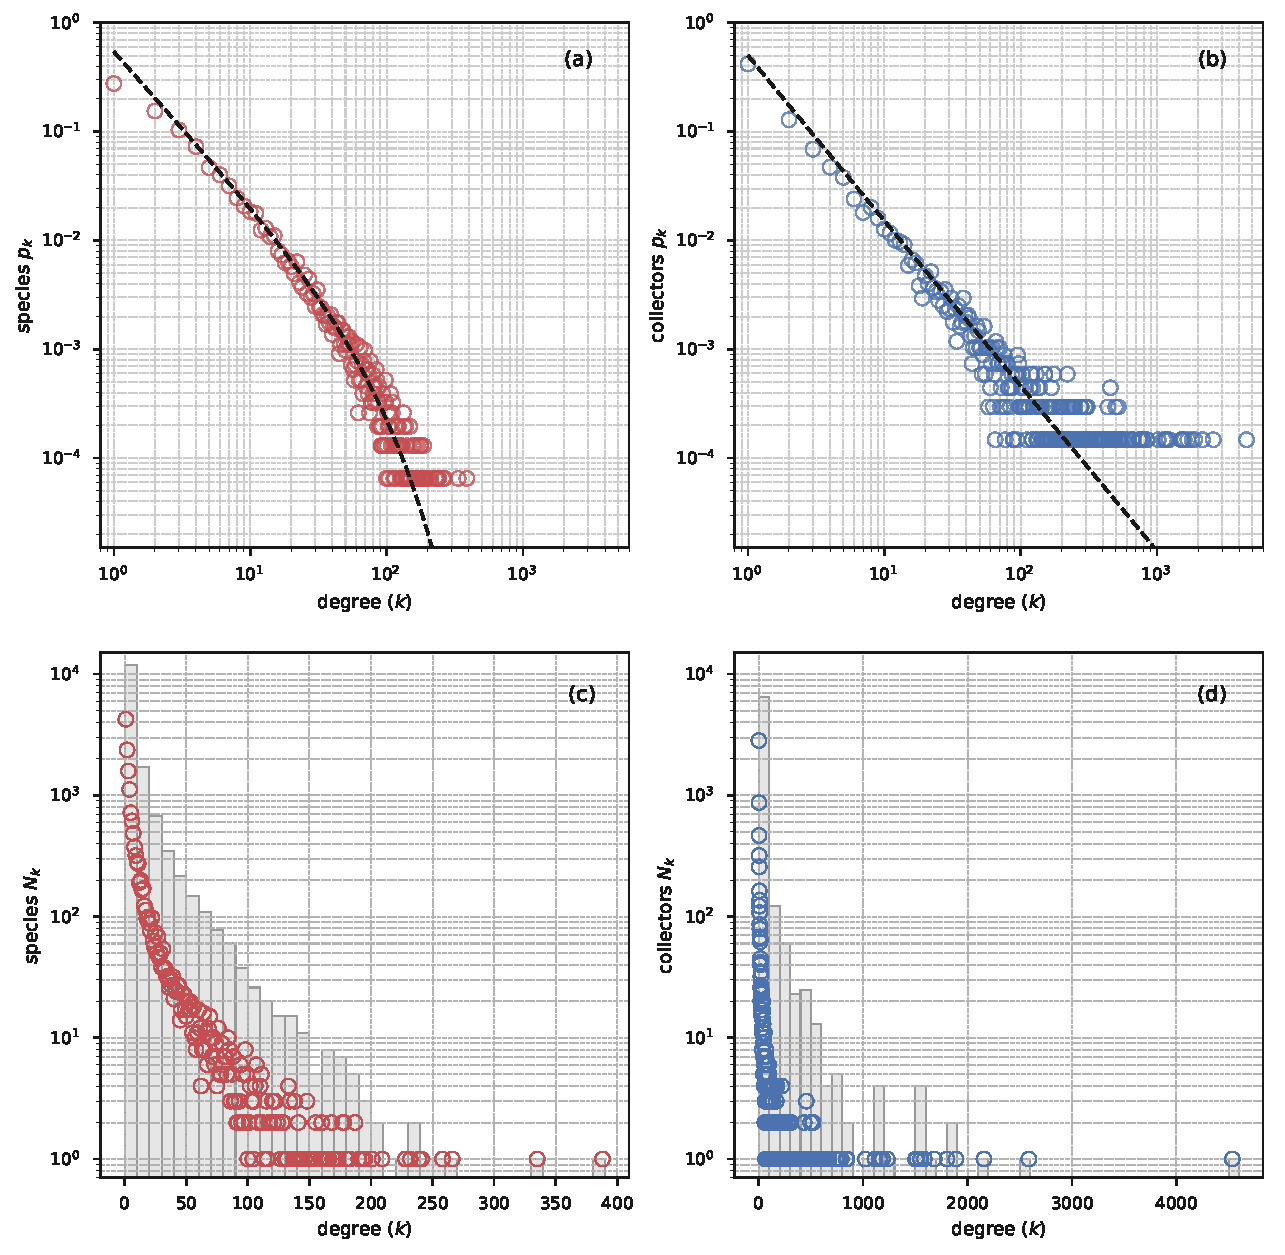
\includegraphics[width=\linewidth]{figures/casestudy_ub/scn_degree_dist}
    \caption{Degree distribution for both species ($a$ and $c$) and collectors ($b$ and $d$) nodes. The upper row plots show the probability $p_k$ of finding nodes with each degree value, using a log-log scale. The dashed curves represent power laws ($a$ has a tail cutoff) that best fit the SCN data, with $\alpha=1.38$ and $\alpha=1.52$ for plots $a$ and $b$, respectively. The exponential cutoff in $a$ is obtained by using $\lambda=0.014$. Plots in the lower row show the total number $N_k$ of nodes with each degree value, using a lin-log scale for enhancing interpretability. Histograms in the background group collectors using bin sizes $s=10$ and $s=100$ for plots $c$ and $d$, respectively.}
    \label{fig:ub_scn_degree_dist}
  \end{figure}
  

As shown in Table \ref{table:ub_scn_degrees}, for collectors nodes $\langle k_{col}\rangle \approx 21.1$, being $\langle k_{col}\rangle$ the average degree calculated for the $S_{col}$ nodes set. This fact can be interpreted as that the number of distinct species a collector has recorded and successfully deposited in the UB herbarium is, in average, approximately $21.1$. Yet, some collectors in the herbarium have recorded much more species than the average, as it is the case of \textit{Howard S. Irwin} (\textit{irwin,hs}), with a total of $4535$ records of distinct species; or \textit{Carolyn E. B. Proença} (\textit{proenca,ceb}), with $1888$ distinct species. Most collectors (around $86.7\%$), however, have degrees below or equal $floor(\langle k_{col} \rangle)$.

For the species nodes set ($S_{sp}$), the average degree $\langle k_{sp}\rangle \approx 9.5$, which can be interpreted as the number of distinct collectors, in average, a species has been collected by. Similarly to nodes in $S_{col}$, most species (around $76.7\%$) have degrees below or equal $floor(\langle k_{sp}\rangle)$, albeit some species have been collected by many more collectors than the average, for example \textit{Myrcia splendens} and \textit{Eugenia punicifolia} (Table \ref{table:ub_scn_degrees}). Those top-10 species are in fact reasonably well-known, common and easily detectable species. Typical from cerrado physiognomies, \textit{Solanum lycocarpum} (\textit{lobeira}), \textit{Palicourea rigida} (\textit{chapéu-de-couro}), \textit{Qualea parviflora} (\textit{pau-terra}) are examples of species that are both very conspicuous and easy to identify.


\begin{table}[t]
\caption{ Some degree metrics for the UB SCN model. For each nodes set the total number of nodes, average degree $\langle k \rangle$, top-10 highest-degree nodes and their respective degrees $k$ are listed. We define $k^*$ as the maximum possible degree of a nodes set, a metric that represents the degree of a hypothetical node which is connected to every single node from the complementary set. Therefore $k/k^*$ is the proportion of nodes from the complementary set a given node is linked to. }
\begin{center}
	\caption{Some degree metrics for the UB SCN model. For each nodes set the total number of nodes, average degree $\langle k \rangle$, top-10 highest-degree nodes and their respective degrees $k$ are listed. We define $k^*$ as the maximum possible degree of a nodes set, a metric that represents the degree of a hypothetical node which is connected to every single node from the complementary set. Therefore $k/k^*$ is the proportion of nodes from the complementary set a given node is linked to.}
  \begin{center}
  \begin{tabular}{l c c c c c}
    & num of nodes & $\langle k \rangle$ & top-10 & $k$ & $k/k^*$ \\
   \hline    collectors & 6768 & 21.08 &
   \begin{tabular}[t]{{@{}c@{}@{}}}irwin,hs\\heringer,ep\\anderson,wr\\proenca,ceb\\ratter,ja\\faria,jeq\\eiten,g\\souza,rr\\harley,rm\\santos,rrb\end{tabular} &
   \begin{tabular}[t]{{@{}c@{}@{}}}4535\\2586\\2156\\1888\\1803\\1681\\1586\\1549\\1514\\1502\end{tabular} &
   \begin{tabular}[t]{{@{}c@{}@{}}}0.30\\0.17\\0.14\\0.12\\0.12\\0.11\\0.10\\0.10\\0.10\\0.10\end{tabular} \\ \\
    species & 15344 & 9.30 &
   \begin{tabular}[t]{{@{}c@{}@{}}}\textit{Myrcia splendens}\\\textit{Myrcia guianensis}\\\textit{Eugenia punicifolia}\\\textit{Casearia sylvestris}\\\textit{Palicourea rigida}\\\textit{Myrcia tomentosa}\\\textit{Qualea parviflora}\\\textit{Solanum lycocarpum}\\\textit{Piper aduncum}\\\textit{Miconia albicans}\end{tabular} &
   \begin{tabular}[t]{{@{}c@{}@{}}}388\\335\\266\\258\\241\\239\\232\\228\\209\\201\end{tabular} &
   \begin{tabular}[t]{{@{}c@{}@{}}}0.06\\0.05\\0.04\\0.04\\0.04\\0.04\\0.03\\0.03\\0.03\\0.03\end{tabular} \\ 
  \hline
  \end{tabular}
  \end{center}
  \label{table:ub_scn_degrees}

\end{center}
\label{table:ub_scn_degrees}
\end{table}

% Check "Analyzing affiliation networks" from Borgatti, in Sage book of social networks analytics
 
%%
%% Projected graphs info


%% Projections degree distribution





% Projections

% Similarity between collectors
% It should be noticed, however, that in practice collectors holding similarity values very close to one tend to be those with very few records in the dataset. More experienced collectors can have higher similarities with some collectors, but it is usually not very high.
%% PLOT max similarity vs degree


%%% QUESTIONS

%% 1. How common are collaborative recordings within the dataset?
%%% What is the proportion of collaborative records in the dataset? How many collaborators
%%% One-collector recording vs >2 collectors recordings
%%% Distribution of team size
%%% Caveats: Some collectors may not include collaborators names in the records

%% x. How likely is a novice collector to become a great collector?

%% x. Do collectors with similar interests tend to collect together?
%%% Mix of the two models
%%% Look for homophily in collectors communities, assortativity.

%% x. Which groups of species best modularize collectors in the dataset, in terms of their collection interests? 
%%% Using SCNs
%%% Are these groups necessarily taxonomic ones (such as family)? Or could functional groups be more relevant in some cases? Or is there a geographical effect?
%%% e.g. Some group might be best classified as specialists on species inhabiting some geographical location, with some specific habit and belonging to some family rather than simply as specialists in a given family.

%% x. The Expert-location problem {Chapt. 8 of book Social Network Data Analytics}
%%% The expert team formation problem: How can we best select experts for a given job, based on how willing they are of collaborating together?
%%% Combine both SCN and CWN
\newcounter{QuestionsCounter}
\setcounter{QuestionsCounter}{1}

\subsubsection*{Question \arabic{QuestionsCounter}: How prevalent are collaborative records?}
blablabla2

\subsubsection*{Question \arabic{QuestionsCounter}: <Another question>}


% References {Newman2004}
% Statistical characterization of SCN structure
%% Species per collectors (species bag), collectors have species signatures
%% Collectors per species
%% Simply projecting this graph originates a very densely-connected network, failing to reveal relevant connectivity patterns (Lambiotte2005)

%% Define finer species taxonomic/functional division that best reflect collectors interests than division by family alone (Lambiotte2005)
%%% Do collectors interests communities reflect taxonomic divisions such as the family level?


% Statistical characterization of CWN structure
%% Largest component, connected components...
%% Assortativity: Do collectors with many collaborators (very collaborative) tend to associate with others that are also very collaborative?

% Network Evolution
%% Is network evolution ruled by preferential attachment?
%% How likely is it that two co-authors of a record will also be co-authors of another one?
%% Do attach influential collectors (high betweeness) attach preferentially to other influential ones? (Goh2003, Newman2004)


\subsection{Degree distribution?}

A first step for characterizing the network is to obtain its degree distribution.
The degree distribution was obtained for both 


\subsection{Who are the most central collectors in this herbarium?}





\subsection{Features Selection}

%% Features engineering



\section{Model Evaluation}


